\section{Flattening the network}

Hierarchical networks are flattened before they are processed by the verification
tools. Flattening produces a new flat network, the original network is not modified.
The algorithm broadly consists of the following three steps:
\begin{enumerate}
 \item Copy the components from the hierarchical network to the flat network.
 \begin{itemize}
  \item For composite objects, the flattener instantiates a copy of the subnetwork
  into the target network. Through recursion of the flattening algorithm, this
  subnetwork is first flattened itself.
 \end{itemize}
 \item Connect the channels between the components in the flat network.
 \item Connect all (flattened) subnetworks
\end{enumerate}


\subsection{Algorithm}
The flattening process uses a recursive algorithm to flatten all composite objects.
Each recursive call takes two parameters: the destination network, which is the same
in all recursive calls, and the source network. In each recursion step, a flat copy
of the source network is inserted into the destination network. The projects root
network is the source network in the first iteration. In subsequent recursion steps,
the subnetworks that define a composite object are used as source networks.

\paragraph{Gates}
In a subnetwork, sources and sinks are used to define the interface between the
subnetwork and the higher-level network. In the flattened network these components
are no longer present. Components in the higher-level network are directly connected
to the components in the subnetwork. Alternatively, when there is a channel between two
composite objects, the components of two subnetworks directly connect to each other.
To prepare for connection of the networks, sources and sinks are replaced during
flattening by temporary components called gates. An XMASSource component gets replaced
by an XMASInGate component. This component has an additional Input port (i\_ext) that
corresponds to the Input port of the composite object in the higher-level network.
Likewise, an XMASSource is converted to an XMASOutGate instance, which has an
additional Output port (o\_ext). Figure~\ref{fig:mc-gates} shows the result.

\begin{figure}[ht]
\includegraphics[width=0.4\textwidth]{my_composite-network}
\hfill
\includegraphics[width=0.5\textwidth]{my_composite-gates}
  \caption{The original composite network (left) and a partial view of the flattened
  network showing the subnetwork with gates (right); the component names have been
  qualified with the composite objects name (mc) to prevent name collisions}
  \label{fig:mc-gates}
\end{figure}


\paragraph{Flattened composite}
The result of a recursion step is a flattened subnetwork. Moreover, the recursion
step generates a number of gates which are still not connected to the external
world. Upon return of a recursive call, these gates are collected and stored in
another temporary component: XMASFlattenedComposite. This component is the direct
equivalent of an XMASComposite in the source network.

\paragraph{Connecting channels}
The second step, connecting the channels between components is easy. Although
composite objects are flattened, the temporary XMASFlattenedComposite objects
are still present. They provide the same interface (Input and Output ports) as
the XMASComposite object in the source network. Connecting to a composite is a
matter of connecting channels to the external ports available on the
XMASFlattenedComposite instances. Even self-connecting composite objects can be
handled this way. Figure~\ref{fig:flattened-composite} details the preceding
two steps.

\begin{figure}[ht]
    \includegraphics[width=0.5\textwidth]{example-hier-network}
    \hfill
    \includegraphics[width=0.5\textwidth]{example-hier-network-inserted}
    \caption{The root network (left) containing a composite object and the
    corresponding flattened network (right) including the XMASFlattenedComposite object}
    \label{fig:flattened-composite}
\end{figure}

\paragraph{Cleaning up}
The final step, per recursion, is to remove the temporary components and gates.
For each flattened composite, all gates are iteratively removed by simply
updating both ports on the opposite ends of the gates ports so that they
directly connect to each other. After this, the XMASFlattenedComposite and its
gates are deleted.


\begin{figure}[ht]
    \centering
    \includegraphics[width=0.5\textwidth]{example-hier-network-final}
    \caption{The resulting flattened network}
    \label{fig:final-network}
\end{figure}




%\paragraph{Gates}
%During flattening of a subnetwork, XMASSources and XMASSinks that represent the
%interfaces of a subnetwork are converted to gates. An XMASSource becomes an
%XMASInGate and an XMASSink becomes an XMASOutGate. Gates are similar to sources
%and sinks but they have an additional port that will be used to connect the gate
%to the external, higher-level network.




%Each recursive call will only create primitives in the destination network. At
%the deepest recursion level, for which the subnetwork contains no composite objects,
%this is simply a matter of copying the primitives*. After the subnetwork has been
%instantiated, one or more interface ports

%Additionally, temporary objects are created to the 

%The flatten function returns a list of all connection points called gates. These
%gates correspond to the sources and sinks in the (sub)network. The 


%The flattening algorithm uses three auxiliary component classes: XMASInGate, XMASOutGate
%and XMASFlattenedComposite. Temporary instances of these classes are created to
%bridge the gap between a subnetwork and the network that contains the composite object.

%* Parameterization of the network!
%Value parameterization: e.g. using a credit-counter with 12 tokens and a credit-counter
%with 5 tokens.

%Structural parameterization: e.g. mesh, spidergon (see proposal)

%\paragraph{XMASFlattenedComposite}
%The actual flattening a composite 
%When a subnetwork has been 
%From the higher-level networks perspective, composites 





%The gates are
%used as interfaces between a subnetwork and the higher-level network. An XMASSource
%component that acts as an input 
%The actual flattening occurs in steps 1 and 3. 

\paragraph{Note:}
While copying a component, all known extensions that a component can have are
copied as well. Which extensions to copy for what component type is currently
hard-coded in the flattener. Ideally, this method will be replaced by a more
generic copying method. Its implementation has been postponed due to changes
required to the underlying bitpowder library. 



